\documentclass{article}
\usepackage[utf8]{inputenc}
\usepackage[T1]{fontenc}
\usepackage[export]{adjustbox}
\usepackage{mathtools,amsthm,amssymb,icomma,upgreek,xfrac,enumerate, enumitem, bbm,titlesec,lmodern,polski,derivative,geometry,multicol,titling,graphicx,url,amsmath,caption,lipsum,float,longtable,booktabs}
\usepackage[table,xcdraw]{xcolor}
\usepackage[hidelinks,breaklinks,pdfusetitle,pdfdisplaydoctitle]{hyperref}
\setlength{\droptitle}{-1cm}
\mathtoolsset{showonlyrefs,mathic}
\title{Testowanie hipotez w rodzinie rozkładów normalnych}
\author{Adam Wrzesiński, Joanna Kołaczek}
\date{18.07.2022}
\newtheoremstyle{break}
{\topsep}{\topsep}%
{\normalfont}{}%
{\bfseries}{}%
{\newline}{}%
\theoremstyle{break}
\newtheorem{zadanie}{Zadanie} 
\newtheorem*{rozwiazanie}{Rozwiązanie}

\titleformat*{\section}{\LARGE\bfseries}
\titleformat*{\subsection}{\Large\bfseries}
\titleformat*{\subsubsection}{\large\bfseries}
\titleformat*{\paragraph}{\large\bfseries}
\titleformat*{\subparagraph}{\large\bfseries}

%% KOMENDY:
\newcommand*{\e}{\mathrm{e}}
\newcommand{\hyline}[2]{%
	$#1$\> --\kern.5em #2 \\}


%% OPERATORY:
% `\diff` od „differential”, czyli odpowiednika słowa „różniczka” w języku
% angielskim.
\DeclareMathOperator{\diff}{d\!}
\newcommand{\indep}{\perp \!\!\! \perp}
\DeclareMathOperator{\EX}{\mathbb{E}}
\newcommand*{\E}{\mathrm{e}}



\begin{document}
	\maketitle
	\newpage
	\tableofcontents
	\clearpage

\numberwithin{equation}{section}

\section*{Wstęp}
	
	Niniejszy raport powstał na potrzeby realizacji laboratorium ze Statystyki Stosowanej, prowadzonych przez dr inż. Aleksandrę Grzesiek, do wykładu dr hab. inż. Krzysztofa Burneckiego. Będziemy testować hipotezy statystyczne dla wartości średniej i wariancji w rodzinie rozkładów normalnych. W tym celu zobrazujemy obszary krytyczne, wyznaczymy p-wartości oraz prawdopodobieństwa wystąpienia błędów I i II rodzaju. Życzymy miłej lektury.


	
\section{Przypadek nieznanej średniej}
Dysponujemy próbą danych z rozkładu $N(\mu,0.2)$. Jej rozkład wizualizujemy za pomocą histogramu (rys. \ref{fig:hist}).
\begin{figure}[H]
	\begin{center}
		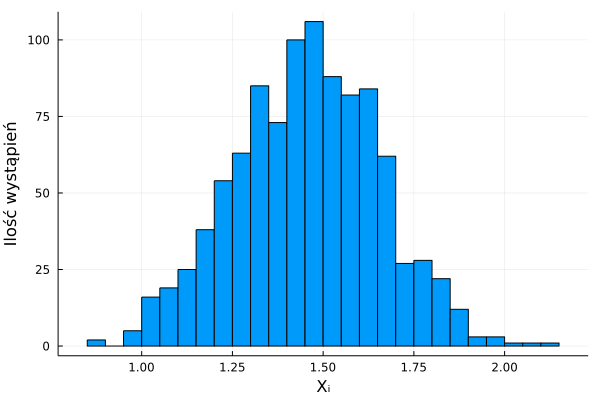
\includegraphics[scale=0.5]{hist1.png}
		\caption{Histogram}
		\label{fig:hist}
	\end{center}
\end{figure}
Nasza hipoteza zerowa to $H_0: \mu_0 = 1.5$. Statystykę testową wyznaczamy ze wzoru (\ref{eq:1}).

\begin{subequations} \label{eq:1}
\begin{equation}
Z = \frac{\bar{X}-\mu_0}{\sigma/\sqrt{n}}.
\end{equation}
\end{subequations}
Jeżeli $H_0$ jest prawdziwa, to $Z\sim N(0,1)$. Aby obliczyć średnią $\bar{X}$ skorzystamy ze wzoru na średną (\ref{eq:2}).
\begin{subequations} \label{eq:2}
\begin{equation}
\bar{X}=\frac{1}{n}\sum\limits_{i=1}^{n}x_i.
\end{equation}
\end{subequations}
W naszym przypadku $\bar{X}=1.455$, $z=-7.041$.
Na poziomie istotności $\alpha = 0.05$ zweryfikujemy kolejne hipotezy alternatywne $H_1$.
\newpage
\subsection{$H_1: \mu \ne \mu_0$}

Zaczynamy od zadania sobie pytania - "Czy rzeczywista średnia jest różna od zakładanej?". Wobec tego średnia może być mniejsza lub większa od podważanej.
Ponieważ gęstość rozkładu standardowego jest funkcją parzystą, to $Z_\alpha = -Z_{1-\alpha}$. Korzystając z tej równości stwierdzamy, że pole pod wykresem na obszarze krytycznym
również dzieli się na dwie połowy. Stąd wnioskujemy, że $p$-wartość jest dwukrotnością pola na dowolej połowie obszaru krytycznego wyznaczanego przez statystykę $z$.
Podsumowując:

	\begin{itemize}
		\item Obszar krytyczny $c=\{x: x\leq -Z_{1-\alpha/2} \lor x\geq Z_{1-\alpha/2}\}$.
		\item p-wartość $p=2P_{H_0}(Z\geq|z|)$
	\end{itemize}
\begin{figure}[H]
	\begin{center}
		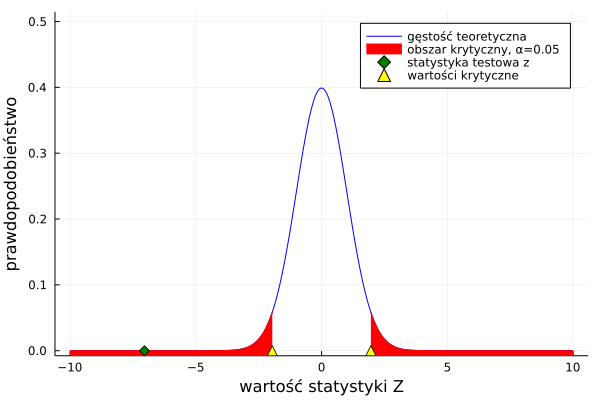
\includegraphics[scale=0.5]{Z1.1.png}
		\caption{Obszar krytyczny na tle gęstości $Z$}
		\label{fig:1}
	\end{center}
\end{figure}
	W naszym przypadku $c=(-\infty,-1.96)\cup (1.96,\infty)$ oraz $p=1.9\cdot 10^{-12}$.\\
	Zaznaczamy na wykresie obszar krytyczny  $c$ oraz statystykę $z$ (rys. \ref{fig:1}). Ponieważ statystyka $z$ znalazła się w obszarze krytycznym możemy przyjąć naszą hipotezę alternatywną $H_1: \mu \ne 1.5$. Ponadto p-wartość jest bardzo mała - prawie zawsze odrzucimy hipotezę zerową.

\newpage
\subsection{$H_1: \mu > \mu_0$}	

Zadajemy pytanie - "Czy rzeczywista średnia jest większa od zakładanej?". Spodziewamy się więc jednostronnego obszaru krytycznego. Upraszcczają się zatem postacie tego obszaru oraz $p$-wartości:

	\begin{itemize}
		\item Obszar krytyczny $c=\{x: x\geq z_{1-\alpha}\}$.
		\item p-wartość $p=P_{H_0}(Z\geq z)$
	\end{itemize}
	\begin{figure}[H]
	\begin{center}
		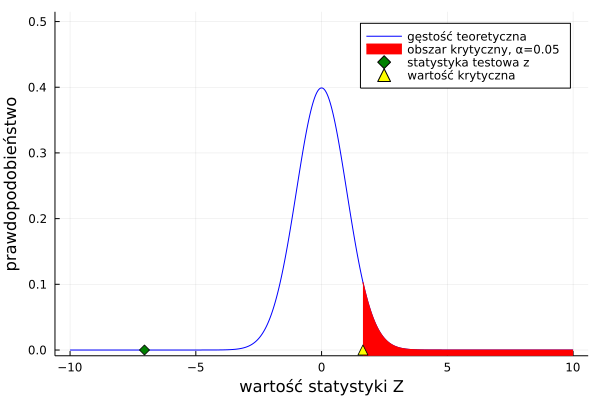
\includegraphics[scale=0.5]{Z1.2.png}
		\caption{Obszar krytyczny na tle gęstości $Z$}
		\label{fig:2}
	\end{center}
	\end{figure}
	W naszym przypadku $c=(1.64,\infty)$ oraz $p=0.999$.\\
	Zaznaczamy na wykresie [\ref{fig:2}]  $c$ oraz statystykę $z$. Ponieważ statystyka $z$ znalazła się poza obszarem krytycznym odrzucamy hipotezę alternatywną, duża p-wartość dodatkowo umacnia nas w przekonaniu, że nie możemy odrzucić hipotezy zerowej.
\newpage
\subsection{$H_1: \mu < \mu_0$}

Ponownie zaczynamy od znalezienia postaci obszaru krytycznego oraz $p$-wartości. Tym razem interesuje nas przedział na lewo od odpowiednich wartości krytycznych:

\begin{itemize}
	\item Obszar krytyczny $c=\{x: x\leq -z_{1-\alpha}\}$.
	\item p-wartość $p=P_{H_0}(Z\leq z)$
\end{itemize}
\begin{figure}[H]
	\begin{center}
		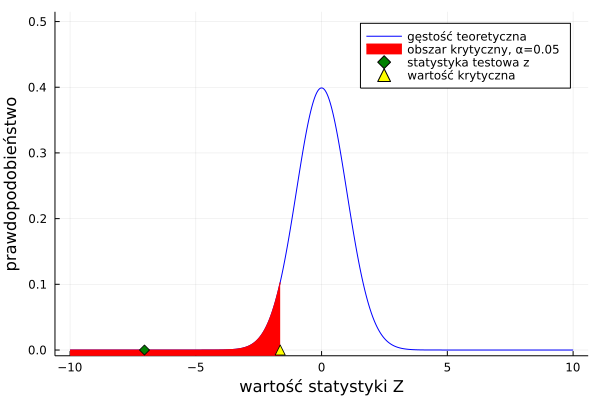
\includegraphics[scale=0.5]{Z1.3.png}
		\caption{Obszar krytyczny na tle gęstości $Z$}
		\label{fig:3}
	\end{center}
\end{figure}
W naszym przypadku $c=(-\infty,-1.64)$ oraz $p=9.51\cdot 10^{-13}$.\\
Sprawdźmy, czy statystyka $z$ znalazła się w obszarze krytycznym $c$  (rys.\ref{fig:3}).  Ponieważ znalazła się ona w obszarze krytycznym odrzucamy hipotezę zerową na korzyść hipotezy alternatywnej. $H_1: \mu < 1.5$. Ponadto p-wartość jest bardzo mała - prawie zawsze odrzucimy hipotezę zerową.\\ \\

\subsection*{Wniosek}
Odrzucamy hipotezę zerową. Z wyjątkowo dużą śmialością stwierdzamy, że rzeczywista średnia jest mniejsza od zakładanej na poziomie istotności $5\%$.
\newpage

\section{Przypadek nieznanej wariancji}
Dysponujemy próbą danych z rozkładu $N(0.2,\sigma^2)$, której rozkład możemy zobaczyć na histogramie (rys. \ref{fig:hist2}).
\begin{figure}[H]
	\begin{center}
		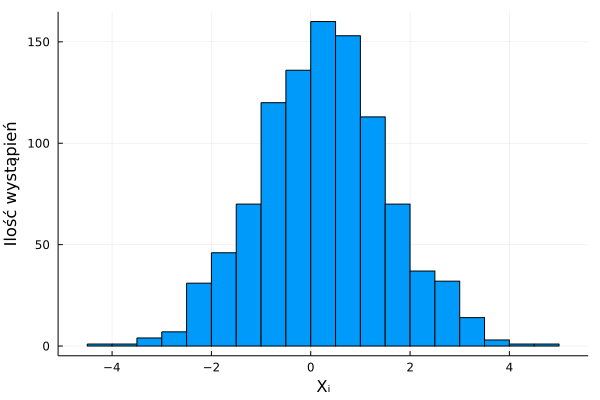
\includegraphics[scale=0.5]{hist2.png}
		\caption{Histogram}
		\label{fig:hist2}
	\end{center}
\end{figure}
Nasza hipoteza zerowa to $H_0: \sigma^2_0 = 1.5$.  Statystykę testową wyznaczamy ze wzoru (\ref{eq:3}).

\begin{subequations} 
\begin{equation}\label{eq:3}
\chi^2 = \frac{(n-1)S^2}{\sigma^2_0},
\end{equation}
\end{subequations}
gdzie $n$ i $S$ to odpowiednio długość oraz wariancja badanej próby.
Jeżeli $H_0$ jest prawdziwa, to $Z\sim \chi^2$z $n-1$ stopniami swobody. Przypomnijmy wzór na wariancję z próbki (\ref{eq:4}).
\begin{subequations} \label{eq:4}
\begin{equation}
S^2=\frac{1}{n-1}\sum\limits_{i=1}^{n}(x_i-\bar{X})^2.
\end{equation}
\end{subequations}

Po podstawieniu do wzorów otrzymujemy $z = 1110.968$ oraz $S^2 =  1.668$. Zweryfikujemy kolejne hipotezy na poziomie istotności $\alpha = 0.05$.

\newpage

\subsection{$H_1: \sigma^2 \ne \sigma^2_0$}

Nie zmenia się za dużo w porównaniu rozdziałem poprzednim. Zamiast standardowego, interesuje nas rozkład $\chi^2$ z $n-1$ stopniami swobody. W związku z tym nie posiadamy już
symetrycznej gęstości. Wobec tego największe zmiany zachodzą dla $p$-wartości. Tym razem jest to dwukrtoność mniejszego pole na lewo lub prawo od niej. Intuicyjnie - jeśli weźmiemy większe pole, to skończymy z prawdopodobieństwem większym od 1, w związku z czym dalsze rozważania byłyby bezsensowne. Podsumowując:

\begin{itemize}
	\item Obszar krytyczny $c=\{x: x^2\leq \chi^2_{\alpha/2,n-1} \lor x^2\geq \chi^2_{1-\alpha/2,n-1}\}$.
	\item p-wartość $p=2min(P_{H_0}(Z\leq z),P_{H_0}(Z\geq z))$
\end{itemize}
\begin{figure}[H]
	\begin{center}
		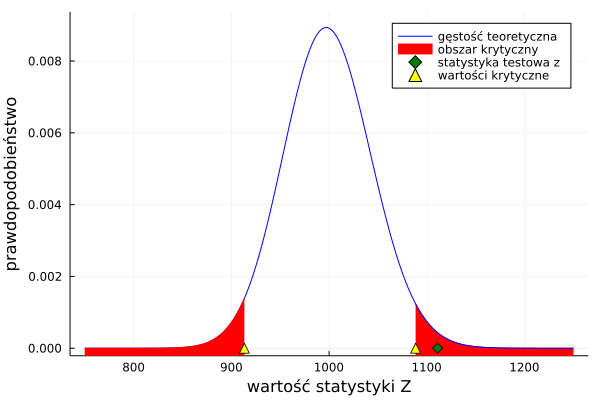
\includegraphics[scale=0.5]{Z2.1.png}
		\caption{Obszar krytyczny na tle gęstości $\chi^2$}
		\label{fig:4}
	\end{center}
\end{figure}
W naszym przypadku $c=[0,~913.3)\cup (1088.487,~\infty)$ oraz $p=0.015$.\\
Zaznaczamy na wykresie [\ref{fig:4}]  $c$ oraz statystykę $z$. Ponieważ statystyka $z$ znalazła się w obszarze krytycznym możemy przyjąć naszą hipotezę alternatywną $H_1: \mu \ne 1.5$. Ponadto p-wartość jest bardzo mała - prawie zawsze odrzucimy hipotezę zerową.
\newpage
\subsection{$H_1: \sigma^2  > \sigma^2_0$}	
Obszary krytyczne oraz $p$-wartość konstruujemy analogicznie względem wcześniejszych rozważań.
\begin{itemize}
	\item Obszar krytyczny $c=\{x: x^2\geq \chi^2_{1-\alpha,n-1}\}$.
	\item p-wartość $p=P_{H_0}(Z\geq z)$
\end{itemize}
\begin{figure}[H]
	\begin{center}
		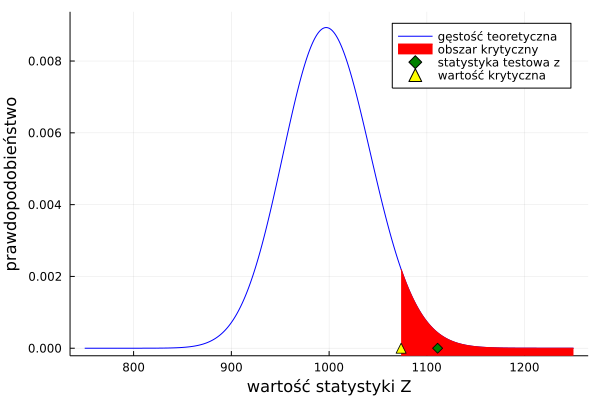
\includegraphics[scale=0.5]{Z2.2.png}
		\caption{Obszar krytyczny na tle gęstości $\chi^2$}
		\label{fig:5}
	\end{center}
\end{figure}
W naszym przypadku $c=[1073.643,\infty)$ oraz $0.008$.\\
Ponieważ statystyka $z$ znalazła się w obszarze krytycznym (rys. \ref{fig:5}) odrzucamy hipotezę zerową na korzyść hipotezy alternatywnej. Ponadto p-wartość jest bardzo mała - prawie zawsze odrzucimy hipotezę zerową.
\newpage
\subsection{$H_1: \sigma^2  < \sigma^2_0$}
\begin{itemize}
	\item Obszar krytyczny $c=\{x: x^2\leq \chi^2_{\alpha,n-1}\}$.
	\item p-wartość $p=P_{H_0}(Z\leq z)$
\end{itemize}
\begin{figure}[H]
	\begin{center}
		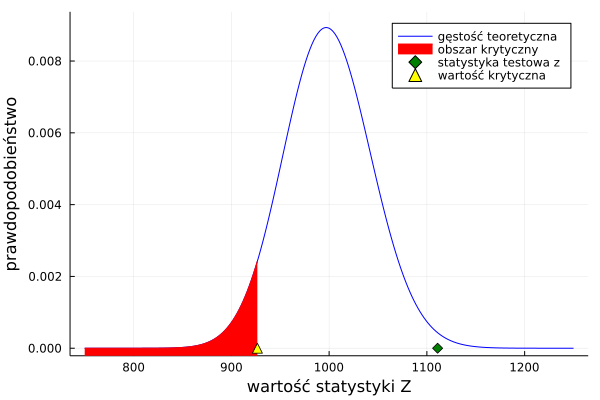
\includegraphics[scale=0.5]{Z2.3.png}
		\caption{Obszar krytyczny na tle gęstości $\chi^2$}
		\label{fig:6}
	\end{center}
\end{figure}
W naszym przypadku $c=[0,~926.631)$ oraz $p=0.992$.\\
Zaznaczamy na wykresie [\ref{fig:6}]  $c$ oraz statystykę $z$. Ponieważ statystyka $z$ znalazła się poza obszarem krytycznym odrzucamy hipotezę alternatywną, duża p-wartość również wskazuje na to, że nie możemy odrzucić hipotezy zerowej.\\ 

\paragraph{Co stanie się kiedy zwiększymy bądź zmniejszymy poziom istotności?} 
W~przypadku zwiększenia poziomu istotności $\alpha$, zwiększy się nasz obszar krytyczny - test stanie się mniej wiarygodny. Zmniejszając poziom istotności, zmniejszamy obszar krytyczny - test jest bardziej wiarygodny. Można zatem powiedzieć, że najbardziej korzystne będzie wybieranie jak najmniejszych $\alpha$ tak aby uniknąć ryzyka odrzucenia prawdziwej hipotezy zerowej. Niestety w praktyce często możemy przeprowadzić tylko ograniczoną ilość badań, eksperymentów, pomiarów, dlatego wybór bardzo małego poziomu istotności nie jest opłacalny. Zwykle przyjmujemy $\alpha=0.05$ (tzn. jesteśmy skłonni popełnić jeden błąd na 20 przypadków). P-wartość nie zależy od poziomu istotności.




\section{Błędy statystyczne}
\textbf{Błąd I rodzaju} - prawdopodobieństwo odrzucenia hipotezy zerowej, gdy ta jest prawdziwa. Jego teoretyczna wartość jest równa pozimowi istotności alpha.\\ \\
\textbf{Błąd II rodzaju} - prawdopodobieństwo przyjęcia fałszywej hipotezy zerowej i odrzucenia prawdziwej hipotezy alternatywnej.\\ \\ 
\textbf{Moc testu} - prawdopodobieństwo uniknięcia błędu drugiego rodzaju.

\subsection*{Przypadek dla nieznanej średniej} 

Symulacyjnie obliczymy prawdopodobieństwa popełnienia błędów I oraz II rodzaju. Wyznaczymy ponadto moc testu. Do pokazania zależności wykorzystamy wykresy pudełkowe, a rozważania będziemy podsumowywać za pomocą tabel.

\subsubsection*{Błąd I rodzaju}

Algorytm:

\begin{enumerate}
\item Ustal poziom ufności $\alpha$, długość $n$ próby losowej $X$ oraz postać hipotezy alternatywnej.
\item Wstaw s = 0.
\item Generuj próbę losową $X$ z rozkładu $N(\mu_0, \sigma)$
\item Wyznacz wartość statystyki testowej $Z$.
\item Wyznacz odpowiedni obszar krytyczny.
\item Sprawdź, czy statystyka $Z$ znalazła się w obszarze krytycznym. Jeśli tak, to zwiększ $s$ o jeden.
\item Powtórz 3-6 $N$ razy.
\item Zwróć $P_I = \frac{s}{N}.$ 
\end{enumerate}


W naszym przypadku $\alpha \in \{0.01, 0.05, 0.1\}$, $n=1000$, hipotezy takie jak omawiane w dwóch poprzednich rozdziałach, $N=1000$.
W celu wykonania boxplotów oraz tabel wykonujemy po 100 symulacji dla każdego przypadku.

\begin{figure}[H]
	\begin{center}
		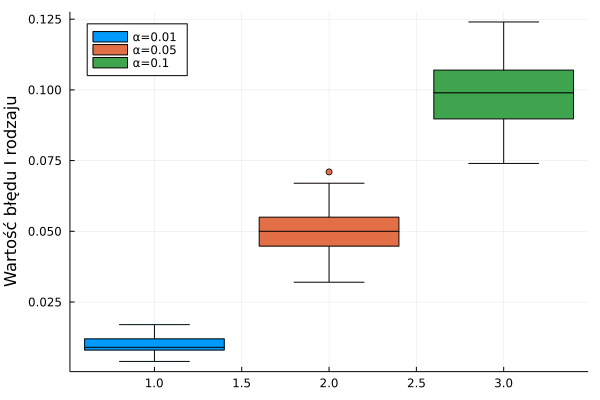
\includegraphics[scale=0.5]{Z3.Irodzaj.png}
		\caption{Błąd I rodzaju w zależności od poziomu istotności $\alpha$}
		\label{fig:7}
	\end{center}
\end{figure}

\begin{table}[H]
	\begin{center}
	\begin{tabular}{|l|l|}
		\hline
		\rowcolor[HTML]{EFEFEF} 
		$\alpha$ & Błąd I rodzaju dla średniej \\ \hline
		0.01 & 0.099                         \\ \hline
		0.05 & 0.049                         \\ \hline
		0.1  & 0.94                         \\ \hline
	\end{tabular}
\caption{Średnia błędu I rodzaju dla 100 symulacji}
\label{table:1}
	\end{center}
\end{table}

Przeprowadzamy symulacje dla prób z rozkładu $N(1.5,~0.2)$ ($H_0: \mu_0 = 1.5$ jest prawdziwa). Widzimy (rys. \ref{fig:7}, tab. \ref{table:1}) że częstość symulacji, w których popełniamy błąd I rodzaju dąży do jego teoretycznej wartości (poziomowi istotności testu). Oznacza to, że algorytm wykorzystany do testowania hipotez działa poprawnie. Popełniamy więc $\frac{1}{\alpha}$ błędów na 100 symulacji.
\newpage
\subsubsection*{Błąd II rodzaju}

Algorytm:

\begin{enumerate}
\item Ustal poziom ufności $\alpha$, średnią $\mu$, odchylenie standardowe $\sigma$, dłuigość $n$ próby $X$  oraz postać hipotezy alternatywnej.
\item Wstaw s = 0.
\item Generuj $X$ z rozkładu $N(\mu, \sigma)$.
\item Wyznacz wartość statystyki testowej $Z$.
\item Wyznacz odpowiedni obszar krytyczny.
\item Sprawdź czy statystyka $Z$ jest poza obszarem krytycznym. Jeśli tak, to zwiększ $s$ o jeden.
\item Powtórz kroki 3-6 $N$ razy.
\item Zwróć $P_{II} = \frac{s}{N}.$
\end{enumerate}

Ustalamy $\alpha = 0.05$, $\mu_0 = 1.5$, $\sigma = 0.2$, $n=1000$ oraz następujące dane:

\begin{itemize}
\item dla $H_1: \mu \ne \mu_0$, $\mu \in \{1.52; 1.51; 1.49; 1.48\},$
\item dla $H_1: \mu > \mu_0$, $\mu \in \{1.51; 1.52; 1.53\},$
\item dla $H_1: \mu < \mu_0$, $\mu \in \{1.49; 1.48; 1.47\}.$
\end{itemize}

Zauważmy (rys. \ref{fig:8}, \ref{fig:9}, \ref{fig:10}, tab. \ref{table:2}), że im bliżej $\mu_0$ znajduje się $\mu$ tym większe prawdopodobieństwo popełnienia błędu II rodzaju, co skutkuje mniejszą mocą testu. Dla naszych danych gdy $|\mu-\mu_0|\geq 0.02$ test zwraca wyniki, które możemy uznać za rzetelne.

\begin{figure}[H]
\begin{multicols}{3}
		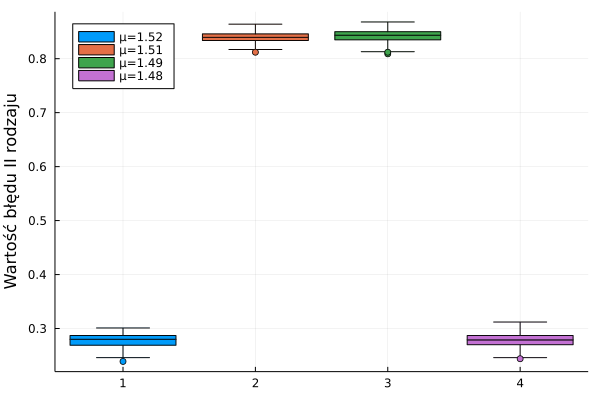
\includegraphics[scale=0.25]{Z3.mu1.png}
		\caption{$H_1: \mu\ne1.5$}
		\label{fig:8}
		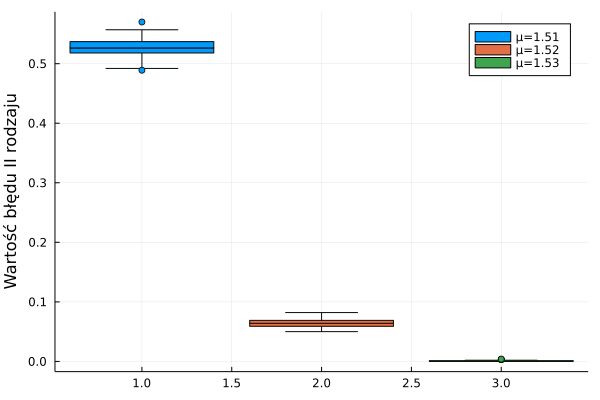
\includegraphics[scale=0.25]{Z3.mu2.png}
		\caption{$H_1: \mu>1.5$}
		\label{fig:9}
		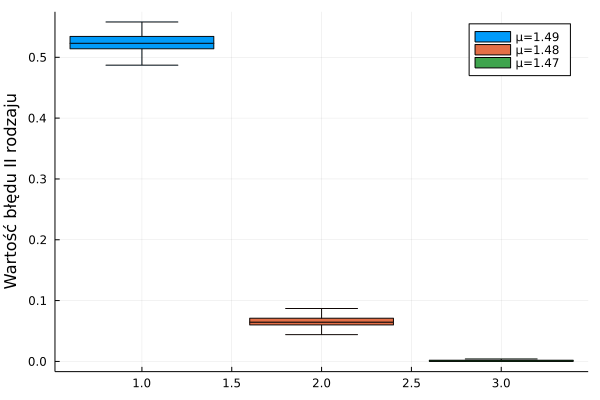
\includegraphics[scale=0.25]{Z3.mu3.png}
		\caption{$H_1: \mu<1.5$}
		\label{fig:10}
\end{multicols}
\end{figure}

\begin{table}[H]
\begin{center}
	\begin{tabular}{|l|l|l|l|}
		\hline
		\rowcolor[HTML]{EFEFEF}
		$H_1$                     & $\mu$   & Błąd II rodzaju dla średniej & Moc testu   \\ \hline
		{$\mu\ne1.5$}            			& 1.52 & 0.280                    & 0.720 \\ \cline{2-4} 
		& 1.51 & 0.839                        & 0.161 \\ \cline{2-4} 
		& 1.49 & 0.843                        & 0.157 \\ \cline{2-4} 
		& 1.48 & 0.279                        & 0.721 \\ \hline
		{$\mu>1.5$} 			& 1.51 & 0.527                        & 0.473 \\ \cline{2-4} 
		& 1.52 & 0.064                        & 0.936 \\ \cline{2-4} 
		& 1.53 & 0.001                        & 0.999 \\ \hline
		{$\mu<1.5$}   			 & 1.49 & 0.523                        & 0.477 \\ \cline{2-4} 
		& 1.48 & 0.065                        & 0.935 \\ \cline{2-4} 
		& 1.47 & 0.001                        & 0.999 \\ \hline
	\end{tabular}
\caption{Średnia błędu II rodzaju dla 100 symulacji}
\label{table:2}
\end{center}
\end{table}

\subsection*{Przypadek dla nieznanej wariancji}

Przeprowadzimy dokładnie takie same symulacje dla tego drugiego przypadku. Zauważmy, że algorytmy są nieomal identyczne jak w przypadku nieznanej średniej. Zmienia się w zasadzie jedynie statystyka testowa i rozkład generowanej próby losowej.
Dane oraz liczbę symulacji przyjmujemy takie same (zamieniamy miejscami średnią i wariancję). Dodatkowo mamy na uwadze, że tym razem drugim parametrem rozkładu normalnego jest wariancja (a nie jak w poprzednim przypadku odchylenie standardowe).

\begin{figure}
	\begin{center}
		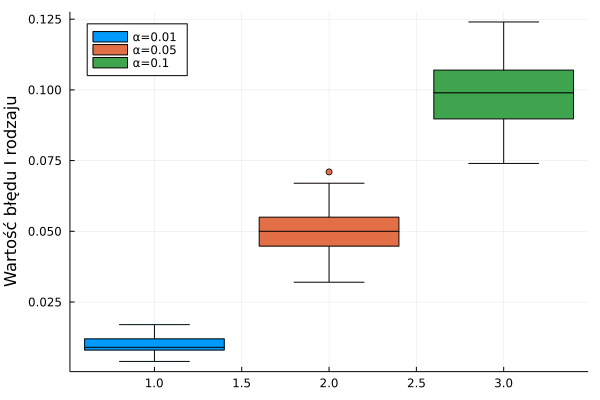
\includegraphics[scale=0.5]{Z3.Irodzaj.png}
		\caption{Błąd I rodzaju w zależności od poziomu ufności $\alpha$}
		\label{fig:11}
	\end{center}
\end{figure}

\subsubsection*{Błąd I rodzaju}


\begin{table}[H]
	\begin{center}
		\begin{tabular}{|l|l|}
			\hline
			\rowcolor[HTML]{EFEFEF} 
			$\alpha$ & Błąd I rodzaju dla wariancji \\ \hline
			0.01 & 0.01                         \\ \hline
			0.05 & 0.049                         \\ \hline
			0.1  & 0.094                         \\ \hline
		\end{tabular}
		\caption{Średnia błędu I rodzaju dla 100 symulacji}
		\label{table:3}
	\end{center}
\end{table}
Po zwizualizowaniu wyników symulacji (rys. \ref{fig:11}, tab. \ref{table:3}) , widzimy że odrzucamy prawdziwą hipotezę zerową w liczbie przypadków bliskiej określonemu teoretycznie poziomowi istotności testu. Oznacza to, że algorytm wykorzystany do testowania hipotez działa poprawnie. Ponownie, popełniamy $\frac{1}{\alpha}$ błędów na 100 symulacji.
\subsubsection*{Błąd II rodzaju}

To samo robimy dla symulacji obliczeń błędu drugiego rodzaju.  Zauważmy (rys. \ref{fig:12}, \ref{fig:13}, \ref{fig:14}, tab.\ref{table:4}), że im bliżej $\sigma_0^2$ znajduje się $\sigma^2$ tym większe prawdopodobieństwo popełnienia błędu II rodzaju, co skutkuje mniejszą mocą testu. Dla naszych $\sigma^2$ moc testu jest bardzo mała - istnieje duża szansa, że odrzucimy prawdziwą hipotezę alternatywną na korzyść fałszywej hipotezy zerowej. \\
\\

\begin{figure}[H]
\begin{multicols}{3}
		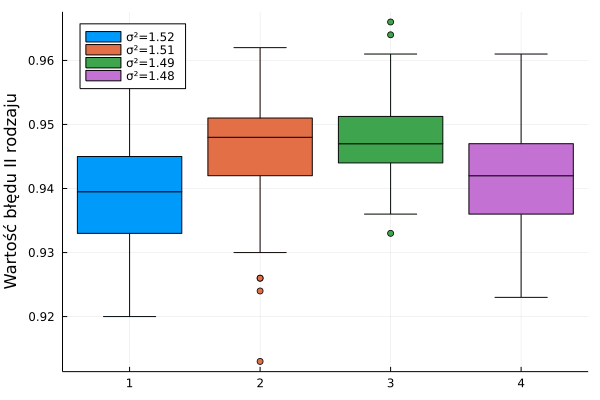
\includegraphics[scale=0.25]{Z3.war1.png}
		\caption{$H_1: \sigma^2\ne1.5$}
		\label{fig:12}
		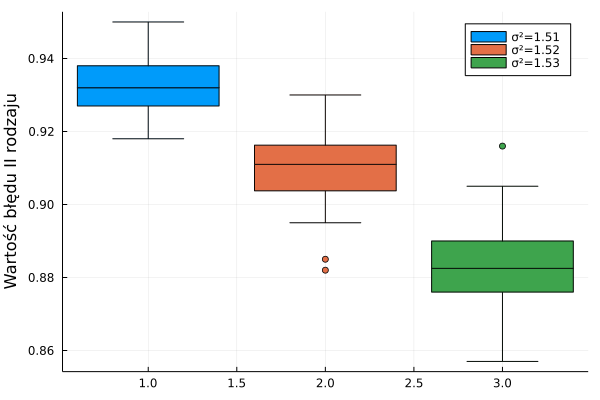
\includegraphics[scale=0.25]{Z3.war2.png}
		\caption{$H_1: \sigma^2>1.5$}
		\label{fig:13}
		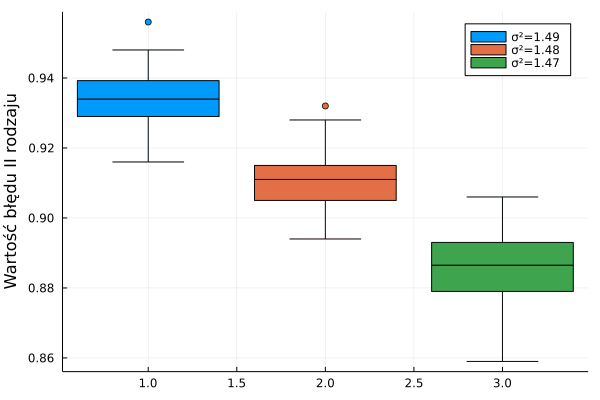
\includegraphics[scale=0.25]{Z3.war3.png}
		\caption{$H_1: \sigma^2<1.5$}
		\label{fig:14}
\end{multicols}
\end{figure}

\begin{table}[H]
	\begin{center}
		\begin{tabular}{|l|l|l|l|}
\hline
\rowcolor[HTML]{EFEFEF} 
$H_1$                               & $\sigma$   & Błąd II rodzaju dla watiancji & moc   \\ \hline
& 1.52 & 0.939                        & 0.061 \\ \cline{2-4} 
& 1.51 & 0.947                        & 0.053 \\ \cline{2-4} 
& 1.49 & 0.947                        & 0.053 \\ \cline{2-4} 
{$\sigma\ne1.5$}             & 1.48 & 0.942                        & 0.058 \\ \hline
& 1.51 & 0.932                        & 0.068 \\ \cline{2-4} 
& 1.52 & 0.911                        & 0.089 \\ \cline{2-4} 
{$\sigma>1.5$} & 1.53 & 0.883                        & 0.117 \\ \hline
& 1.49 & 0.934                        & 0.066 \\ \cline{2-4} 
& 1.48 & 0.911                        & 0.089 \\ \cline{2-4} 
{$\sigma<1.5$}    & 1.47 & 0.887                        & 0.113 \\ \hline
		\end{tabular}
		\caption{Mediana błędu II rodzaju dla 100 symulacji}
		\label{table:4}
	\end{center}
\end{table}

\end{document}